% Created 2017-10-29 Sun 11:00
\documentclass[11pt]{article}
\usepackage[utf8]{inputenc}
\usepackage[T1]{fontenc}
\usepackage{fixltx2e}
\usepackage{graphicx}
\usepackage{longtable}
\usepackage{float}
\usepackage{wrapfig}
\usepackage{rotating}
\usepackage[normalem]{ulem}
\usepackage{amsmath}
\usepackage{textcomp}
\usepackage{marvosym}
\usepackage{wasysym}
\usepackage{amssymb}
\usepackage{hyperref}
\tolerance=1000
\usepackage[left=1in,right=1in,top=1in,bottom=1in]{geometry}
\usepackage{amsmath}
\date{October 30, 2017}
\title{Week 10 lecture notes - PSYC 5316}
\hypersetup{
  pdfkeywords={},
  pdfsubject={},
  pdfcreator={Emacs 25.2.1 (Org mode 8.2.10)}}
\begin{document}

\maketitle
Last week, we introduced Bayesian modeling through sampling the posterior.  This week, we will finish up our discussion of the modeling process by talking about using the model for \textbf{prediction}.

\section*{Evaluating Bayesian models}
\label{sec-1}
Last week, our computations gave us information about the plausible values of $p$ for our binomial model.  For example, we computed an 80\% HPDI for $p$ to be [0.47,0.83], which means that $p$ lies between 0.47 and 0.83 with probability 0.80.  In fact, we estimate the entire posterior distribution (i.e., the probability values for \textbf{all} $p$ between 0 and 1).

We can now take this information and "go the other way".  That is, we can use the estimated parameter values $p$ and estimate how likely a given data observation would be.  That is, our model is \emph{generative} in the sense that we can generate predictions from the model.

To illustrate, let's assume that $p=0.7$.  The following R code will perform 1000 simulations of our experiment (as a reminder, remember that we started with the game of tossing a globe 9 times and recording W or L..the \texttt{rbinom} will count the number of "successes" as water landings). Then, we'll plot a very simple type of histogram to show the relative frequency of each possible number of outcomes (0-9).

\begin{verbatim}
predictions = rbinom(1000, size=9, prob=0.7)
plot(table(predictions), xlim=c(0,9))
\end{verbatim}

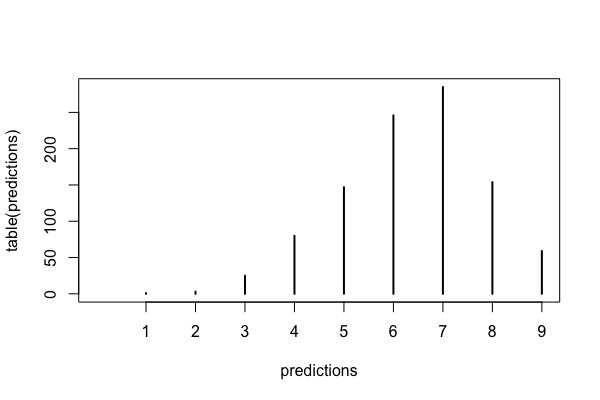
\includegraphics[width=.9\linewidth]{figures/week9/predict1.jpeg}

Note that with $p=0.7$, we still get quite a large range of possible outcomes.  However, the outcomes $x=6$ and $x=7$ are still the most frequent (as we would expect, since 70\% of 9 is 6.3).

As an exercise, you should play around with different values of $p$, ranging from small values (e.g., $p=0.1$) to larger values (e.g., $p=0.9$).  What changes about the distribution of predictions?  

The R code below will show how the distribution of predictions changes for $p$ from 0.1 to 0.9:

\begin{verbatim}
par(mfrow=c(1,5))
Ps = c(0.1,0.3,0.5,0.7,0.9)
for (i in 1:5){
  predictions = rbinom(1000, size=9, prob=Ps[i])
  plot(table(predictions), xlim=c(0,9), ylab="", main=paste("p=",Ps[i]))
}
par(mfrow=c(1,1))
\end{verbatim}

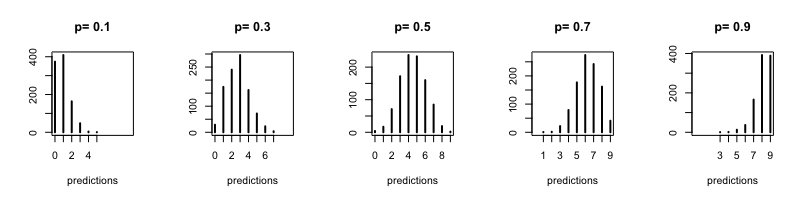
\includegraphics[width=.9\linewidth]{figures/week9/predictive.png}

However, our estimate for $p$ is a \emph{distribution} of values..not a single value.  Thus, we need to incorporate our uncertainty for $p$ in our prediction as well.  The way to do this is through the \textbf{posterior predictive} distribution. 

Basically, the idea is as follows.  From the figure above, we can see that as $p$ increases from 0 to 1, the peak of the predictive distribution shifts from the low end $x=1$ to the high end $x=9$.  However, from our posterior distribution of $p$, we know that the probability that $p$ lies on either of these ends is very small.  Thus, we need to incorporate this knowledge into our predictive distribitution.  

Essentially, we need to form a \emph{weighted average} of predictions.  Predicted observations on the low end ($x=0,1$) come from small values of $p$, which are not very common in our posterior distribution.  Similarly, predicted observations on the high end ($x=8,9$) come from large values of $p$, which are also not very common in the posterior distribution.  When we weight the likelihood of the various observations by the relative posterior probabilities for $p$, we get a result that we call the \textbf{posterior predictive distribution}.  The math can be complicated, but the R code is simple:

\begin{verbatim}
predictions = rbinom(1000, size=9, prob=samples)
plot(table(predictions), xlim=c(0,9))
\end{verbatim}

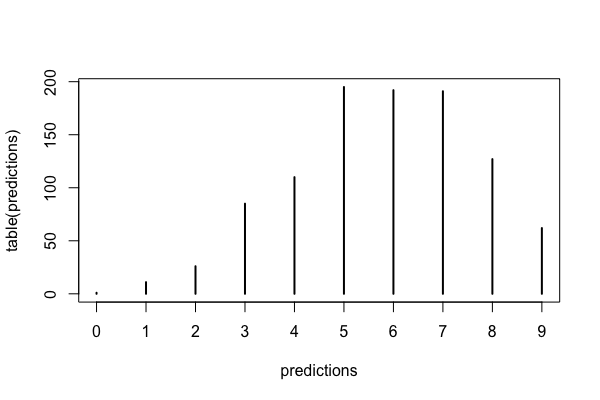
\includegraphics[width=.9\linewidth]{figures/week9/postPredictive.png}

Notice how the only bit of code that we changed is the \texttt{prob} value.  In the above samples, we used a fixed value of $p$.  In the posterior predictive distribution, we set $p$ to be a random variable that is shaped like our posterior distribution for $p$.  Since we approximated this distribution with \texttt{samples} earlier, we can simply set \texttt{prob=samples} to accomplish this.

Notice how the posterior predictive distribution peaks around 6, which matches with our observed data (remember, we saw $x=6$ water landings in our example).  Thus, we can conclude that the model is adequate in the sense that it predicts what we've already seen.  This predictive adequacy is a fundamental part of Bayesian modeling, and it is called a \textbf{posterior predictive check}.

\section*{Next step: MCMC sampling}
\label{sec-2}
So far, we have talked about how to construct a Bayesian model. We can summarize this into the following steps:

\begin{enumerate}
\item We begin with a \emph{data story}; that is, we hypothesize a process by which our data might have arisen.  This results in a \emph{likelihood} function.
\item We then decide on a prior, which represents our prior knowledge.
\item Then, we use Bayes theorem to update our model by \emph{feeding} it the data. Technically, this amounts to computing a \emph{posterior} by multiplying the prior and the likelihood.  Computationally, we use \emph{sampling} to accomplish this.
\item Once we estimate our posterior distribution, we check our model by generating a \emph{posterior predictive distribution}, which incorporates both data uncertainty as well as parameter uncertainty into a single distribution.  We compare this posterior predictive distribution to our observed data; if the observed data match what we would \emph{expect} from the model (based on the posterior predictive), we can conclude that our model does an adequate job of describing our data.
\end{enumerate}

We will finish our intro to Bayesian modeling by discussing a more modern method of posterior sampling known as \textbf{Markov chain Monte Carlo} sampling.

\section*{The Metropolis algorithm}
\label{sec-3}

MCMC methods work by taking random samples from the posterior.  The MCMC method we will discuss is called the \textbf{Metropolis algorithm}.  It works by taking posterior samples in such a way that more time is spent wherever the posterior distribution is more dense.  In the long run (i.e., after many steps), the distribution of samples will then form a very good approximation to the actual posterior distribution.

To illustrate how the algorithm works, I take the approach used by Richard McElreath and describe a fictional story involving a king who wishes to travel around the islands in his kingdom.

King Markov ruled over an archipelago consisting of 10 islands, each arranged in a circle.  His main obligation was that the time spend visiting the people of each island should be proportional to the population of the island.  That is, if island 1 had twice as many people as island 2, then he should spend twice as many days on Island 1 as compared to Island 2.

An easy way to accomplish this would be to simply have a list of each Island's population.  However, the king had no use for such trivialities, and thus required his cabinet to develop a daily travel plan that would satisfy his obligation without having to remember or write down any island's population.

Senator Metropolis (an esteemed member of the cabinet who is also a very capable applied mathematician) developed the following algorithm:

\begin{enumerate}
\item Whereever the King is, each week he needs to decide between staying put for another day, or moving to one of the two adjacent islands.  To decide his next move, he flips a coin.

\item If the coin turns up heads, the King \emph{considers} moving to the adjacent island \emph{clockwise}.  If it turns up tails, he considers moving \emph{counterclockwise}.  This is called the \emph{proposal} island.

\item To decide whether he moves to the proposal island, he uses a rather interesting random sampling procedure.  He collects a number of white stones to represent the population of the \emph{current} island, and a number of black stones to represent the population of the \emph{proposal} island.  Then, he does the following:
\begin{itemize}
\item if the number of black stones exceeds the number of white stones (that is, the relative population of the proposal island is larger than the current island), he \emph{always} moves to the proposal island.
\item if the number of black stones is less than the number of white stones, he, he removes a number of white stones equal to the number of black stones.  For example, if he had 4 black stones and 6 white stones, we would then remove 4 white stones to end with 2 white stones.  In other words, the ratio of black/white stones would be 4:2.
\item finally, he reaches into the bag and pulls a stone.  If it is black, he moves to the proposal island.  If it is white, he stays.
\end{itemize}
\end{enumerate}

Believe it or not, this algorithm works!  To get the hang of it, we will try it in class for a few cycles. Then, we will use R to see how the algorithm works in the long run.

The following series of R code cunks will demonstrate the long-run behavior.

First, we define the population of each island. This is entirely arbitrary, and I invite you to play around with the values in \texttt{population}.

\begin{verbatim}
islandNumber = 1:10
populations = c(2,3,3,5,6,10,10,1,2,3)
plot(islandNumber, populations, type="h")
\end{verbatim}

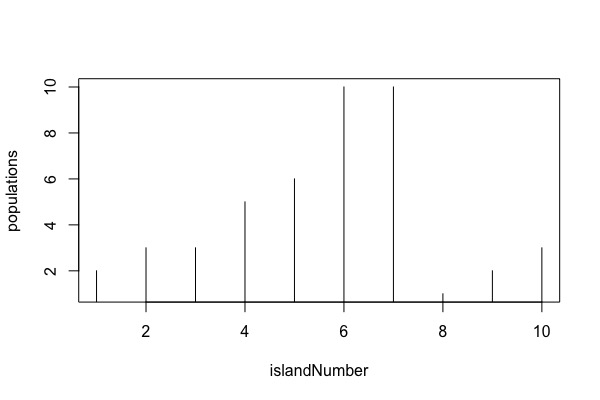
\includegraphics[width=.9\linewidth]{figures/week10/islandPop.jpeg}

Now the algorithm is instantiated below.  Please try to read the code in light of the algorithm as presented above.  The key is that there is a random proposal island selected, and then we have to decide whether to "stay" or "go", which is done by a "coin flip" that is biased to come up heads according to the ratio of population densities (the so-called "acceptance ratio").

(also note that there is an extra step for THIS situation whereby we need to make the island chain circular..this won't be relevant to any other of the situations we talk about..it is simply to make this example work!)

\begin{verbatim}
# begin recording locations
N=10000
locations = numeric(N)
locations[1] = sample(1:10,1) # random starting place

# loop that defines Metropolis algorithm
for (i in 2:N){
  # take random walk either left or right
  proposal = locations[i-1] + sample(c(-1,1), 1)
  
  # make chain of islands circular
  if (proposal==11){proposal=1}
  if (proposal==0){proposal=10}
  
  # compute acceptance ratio (ratio of pop densities)
  current = populations[locations[i-1]]
  proposed = populations[proposal]
  acceptRatio = min(1, proposed/current)
  
  # move or stay according to acceptance ratio
  makeStep = rbinom(1, size=1, prob=acceptRatio)
  if (makeStep==0){
    locations[i]=locations[i-1]
  }
  else{
    locations[i]=proposal
  }
}

plot(locations[1:100])
plot(table(locations))
\end{verbatim}

The two plots at the end show us that everything worked.  First, we plot the first 100 days worth of samples:

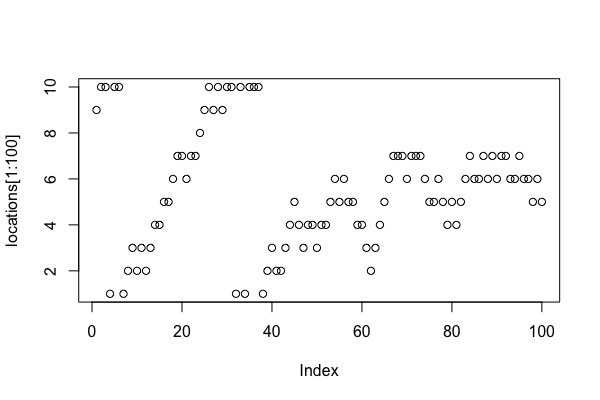
\includegraphics[width=.9\linewidth]{figures/week10/samples.jpeg}

Next, we plot the proportion of time spent on each island.  Notice how it closely resembles the original population density plot above.  Magic!

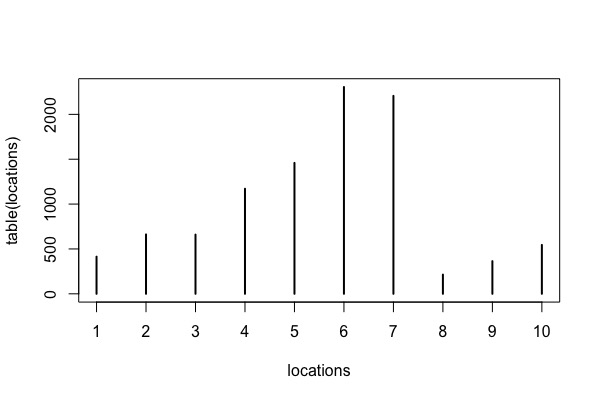
\includegraphics[width=.9\linewidth]{figures/week10/sampledPop.jpeg}
% Emacs 25.2.1 (Org mode 8.2.10)
\end{document}